\documentclass[english]{jflart}
\usepackage[utf8]{inputenc}
\usepackage[T1]{fontenc}
\usepackage{minted}
\usepackage{etoolbox,xpatch}
\usepackage{ tipa }
\usepackage{float}
\usepackage[normalem]{ulem}
\usepackage[backend=biber, style=alphabetic]{biblatex}
\usepackage{newunicodechar}
%\usepackage[section]{placeins}
\addbibresource{bibliography.bib}

% Numéro et année des JFLAs visées par l'article, obligatoire.
\jfla{35}{2024}

\title{Destination-passing style programming: a Haskell implementation}
% Un titre plus court, optionnel.
%\titlerunning{Du bon usage de~\texttt{jflart.cls}}

% Auteurs, liste non abrégée.
\author[1]{Thomas Bagrel}
% \author[2]{Cunégonde Martin}
% \author[2]{Odoacre Contempierre}
% Une liste d'auteurs abrégée à utiliser à l'intérieur de l'article.
\authorrunning{Bagrel}

% Affiliations des auteurs
\affil[1]{INRIA/LORIA, Vand\oe{}uvre-lès-Nancy, 54500, France}
\affil[1]{TWEAG, Paris, 75012, France}

% Une commande définie par l'utilisateur
\newcommand{\cmd}[1]{\texttt{\textbackslash {#1}}}
\newcommand{\mpar}{\text{\,\textramshorns\,}}
\newcommand{\dest}{-\prec}
\newcommand{\TODO}[1]{{\color{red}\large #1}}
\newcommand{\mnew}[1]{\colorbox{green}{#1}}
\newcommand{\muline}[1]{\uline{#1}}
\newcommand{\mold}[1]{\colorbox{red}{#1}}
\newunicodechar{⊸}{\ensuremath{\multimap}}
\newunicodechar{→}{\ensuremath{\to}}
\newunicodechar{⇒}{\ensuremath{\Rightarrow}}
\newunicodechar{;}{\textbf{\large;}}
\newunicodechar{∀}{\ensuremath{\forall}}
\makeatletter
\AtBeginEnvironment{minted}{\dontdofcolorbox}
\def\dontdofcolorbox{\renewcommand\fcolorbox[4][]{##4}}
\xpatchcmd{\inputminted}{\minted@fvset}{\minted@fvset\dontdofcolorbox}{}{}
\xpatchcmd{\mintinline}{\minted@fvset}{\minted@fvset\dontdofcolorbox}{}{} % see https://tex.stackexchange.com/a/401250/
\makeatother

\begin{document}

\maketitle

\begin{abstract}
Destination-passing style programming introduces destinations, which represents the address of a write-once memory cell. Those destinations can be passed around as function parameters, and thus enable the caller of a function to keep control over memory management: the body of the called function will just be responsible of filling that memory cell. This is especially useful in functional programming languages such as Haskell, in which the body of a function is typically responsible for allocation of the result value.

Programming with destination in Haskell is an interesting way to improve performance of critical parts of some programs, without sacrificing memory warranties. Indeed, thanks to a linearly-typed API we designed, a write-once memory cell cannot be left uninitialized before being read, and is still disposed of by the garbage collector when it is not in use anymore, eliminating the risk of uninitialized read, memory leak, or double-free errors that can arise when memory is handled manually.

With the implementation of destinations for Haskell through compact regions we provide in this article, we reach a 15-40\% improvement over memory allocation in a simple parser example, and 0-50\% improvement in run time. We also provide a few examples of programs that can be implemented in a tail-recursive fashion thanks to destinations, which is crucial for performance in strict contexts.

Safety proofs for the API are not provided in this article though, and will be the subject of a future article.
\end{abstract}

\tableofcontents{}

\TODO{[] Link repo?}\\

\section{Introduction}

Destination-passing style (DPS) programming takes its source in the early days of imperative languages with manual memory management. In the C programming language, it's quite common for a function not to allocate memory itself for its result, but rather to receive a reference to a memory location where to write its result (often named \emph{out parameter}). In that scheme, the caller of the function has control over allocation and disposal of memory for the function result, and thus gets to choose where the latter will be written.

DPS programming is an adaptation of this idea for functional languages, based on two core concepts: having arbitrary data structures with \emph{holes} --- that is to say, memory cells that haven't been filled yet --- and \emph{destinations}, which are references to the location of those holes. A destination can be passed around, as first-class object of the language (unlike holes), and it allows remote action on one hole of a structure: when one \emph{fills} the destination with a value, that value is in fact written in the associated hole. Because structures are allowed to have holes, they can be built from the root down, rather than from the leaves up. Indeed, children of a parent node no longer have to be specified when the parent node is created; they can be left empty (which leaves holes in the parent node), and added later through destinations to those holes. It is thus possible to write very natural solutions to problems for which the usual functional bottom-up building approach is ill-fitting. In addition to better expressiveness, DPS programming can also lead to better time and/or space performance for critical parts of a program.

That being said, DPS programming is not about giving unlimited manual control over memory or using mutations without restrictions. The existence of a destination is directly linked to the existence of an accompanying hole: we say that a destination is \emph{consumed} when it has already been used to write something in its associated hole. It must not be reused after that point, to ensure immutability and prevent a range of memory errors.

In this paper, we design a destination API whose memory safety (write-once model) is ensured through a linear type discipline. Linear types systems are based on Girard's Linear logic~\cite{girard_linear_1995}, and introduce the concept of \emph{linearity}: one can express through types that a function will \emph{consume} its argument exactly once given the function result is \emph{consumed} exactly once too. Linearity helps to manage resources --- such as destinations --- that one should not forget to \emph{consume} (e.g. forgetting to fill a hole before reading a structure), but also that shouldn't be reused several times.

The Haskell programming language is equipped with support for linear types through its main compiler, \emph{GHC}, since version 9.0.1~\cite{bernardy_linear_2018}. But Haskell is also a \emph{pure} functional language, which means that side effects are only safe to produce inside monadic functions. This led us to set a slightly more refined goal: we wanted to hide impure memory effects related to destinations behind a \emph{pure} Haskell API, and make the whole safe through the linear type discipline. Although the theoretical proofs of type safety haven't been made yet, the early practical results seem to indicate that we achieved that goal despite the technical challenges that arose. The purity of the final API makes it very practical to partially adopt DPS programming in a codebase (compared to a monadic API which would be more ``contaminating'').

Section~\ref{sec:motivating-examples} of this paper presents three common problems which benefit greatly from a DPS-based implementation --- for either a performance or expressiveness reason. Section~\ref{sec:api} focuses on the design of a type-safe API to handle destinations in a language equipped with linear types. Then, section~\ref{sec:implementation} details how we tackled the implementation of the DPS API with/inside GHC, and the couple of challenges that arose. Finally, section~\ref{sec:benchmark} presents benchmarks for the various implementations shown in section~\ref{sec:motivating-examples} as well as implementations of the \mintinline{haskell}`map` function based on destinations.

\subsection{Preliminary notions about linear types and destinations in Haskell}\label{ssec:intro-linearity}

Linear Haskell~\cite{bernardy_linear_2018} introduces the linear function arrow, \mintinline{haskell}`a ⊸ b`, that guarantees that the argument of the function will be consumed exactly once when the result of the function is consumed exactly once. On the other hand, the regular function arrow \mintinline{haskell}`a → b` doesn't guarantee how many times its argument will be consumed when its result is consumed once.

A value is said to be \emph{consumed once} (or \emph{consumed linearly}) when it is pattern-matched on and its sub-components are consumed once; or when it is passed as an argument to a linear function whose result is consumed once. A function is said to be \emph{consumed once} when it is applied to an argument and when the result is consumed exactly once too. Linearity on functions arrows creates a chain of dependency/trust about consumption of values, which is usually bootstrapped by using scope-passing style, as detailed in section~\ref{ssec:api-linearity}.

Linear Haskell introduces a wrapper named \mintinline{haskell}`Ur` that serves to indicate that a value in a linear context doesn't have to be consumed linearly. The type \mintinline{haskell}`Ur a` is equivalent to $!a$ in linear logic, and there is an equivalence between \mintinline{haskell}`Ur a ⊸ b` and \mintinline{haskell}`a → b`.

The value \mintinline{haskell}`(x, y)` is said to be consumed linearly only when both \mintinline{haskell}`x` and \mintinline{haskell}`y` are consumed exactly once; whereas \mintinline{haskell}`Ur x` is considered to be consumed once as long as one pattern-match on it, even though \mintinline{haskell}`x` is not consumed exactly once (it can be consumed several times or none at all). Conversely, if \mintinline{haskell}`x` and \mintinline{haskell}`y` are said to be used linearly when one constructs \mintinline{haskell}`(x, y)`, \mintinline{haskell}`x` is not considered as consumed linearly when one builds \mintinline{haskell}`Ur x`. As a result, only values already wrapped in \mintinline{haskell}`Ur` or coming from the left of a non-linear function arrow \mintinline{haskell}`→` can be put in another \mintinline{haskell}`Ur` without breaking linearity. The only exceptions are types which implement the \mintinline{haskell}`Movable` typeclass such as \mintinline{haskell}`Int` or \mintinline{haskell}`()`. That typeclass provides \mintinline{haskell}`move :: a ⊸ Ur a` so a value can escape from linearity restrictions.

Destinations are represented by the type \mintinline{haskell}`Dest a`, where \mintinline{haskell}`a` stands for the type of the associated hole. \mintinline{haskell}`Dest`s are meant to be managed linearly, and thus doesn't implement \mintinline{haskell}`Movable`.

\paragraph{Operators}

Two uncommon operators are often used in the rest of this article:
\begin{itemize}
  \item \mintinline{haskell}`(<&>) :: Functor f => f a ⊸ (a ⊸ b) ⊸ f b` is the same as \mintinline{haskell}`fmap` with the order of the arguments flipped: \mintinline{haskell}`i <&> (\d → f d) = fmap (\d → f d) i`. It will be used to map over the destinations \mintinline{haskell}`d` associated to an incomplete data structure \mintinline{haskell}`i`;
  \item \mintinline{haskell}`(;;) :: () ⊸ b ⊸ b` is used to chain a linear operation returning \mintinline{haskell}`()` with one returning a value of type \mintinline{haskell}`b` without breaking linearity.
\end{itemize}

\section{Motivating examples for destination-passing style programming}\label{sec:motivating-examples}

\subsection{Efficient difference lists}\label{ssec:dlist}

Linked lists are a staple of functional programming, but they aren't efficient for concatenation, especially when the concatenation calls are nested to the left.

In an imperative context, it would be quite easy to concatenate linked lists efficiently. One just have to keep both a pointer to the root and to the last \emph{cons} cell of each list. Then, to concatenate two lists, one just have to mutate the last \emph{cons} cell of the first one to point to the root of the second list.

It isn't possible to do so in an immutable functional context though. Instead, \emph{Difference lists} can be used: they are structures that are fast to convert into lists ($\mathcal{O}(1)$ amortized) and tend to emulate the idea of having a mutable (here, write-once) last \emph{cons} cell. Usually, a difference list \mintinline{haskell}`[x1, ..., xn, ?]` is encoded by a function taking a last element \mintinline{haskell}`ys` of type \mintinline{haskell}`[a]` and returning \mintinline{haskell}`x1 : ... : xn : ys` (having type \mintinline{haskell}`[a]` too).

With such representation, concatenation is just function composition: \mintinline{haskell}`f1 <> f2 = f1 . f2`, and we have \mintinline{haskell}`mempty = id`\footnote{\mintinline{haskell}`mempty` and \mintinline{haskell}`<>` are the standard notations for the neutral element and internal operation of a monoid in Haskell}, \mintinline{haskell}`toList f = f []` and \mintinline{haskell}`fromList xs = \ys → xs ++ ys`.

In DPS, instead of encoding the concept of a write-once hole with a function, we can represent the hole as a first-class object with a \emph{destination}. A difference list now become an actual data structure in memory --- not just a pending computation --- that has two handles: one to the root of the list of type \mintinline{haskell}`[a]`, and one to the yet-to-be-filled hole in the last cons cell, represented by a destination of type \mintinline{haskell}`Dest [a]`.

With the function encoding, it isn't possible to read the list until a last element of type \mintinline{haskell}`[a]` have been supplied to complete it. With the destination representation, this constraint must persists: the actual list \mintinline{haskell}`[a]` shouldn't be readable until the accompanying destination is filled (or \emph{linearly consumed}, as we sometimes write), otherwise memory safety wouldn't be respected. This constraint is embodied by the \mintinline{haskell}`Incomplete a b` type of our destination API: \mintinline{haskell}`b` is what needs to be linearly consumed to make the \mintinline{haskell}`a` readable. Most of the time, the \mintinline{haskell}`b` side carries the destinations of the structure. A difference list is then \mintinline{haskell}`type DList a = Incomplete [a] (Dest [a])`: one should fill the \mintinline{haskell}`Dest [a]` (with a \mintinline{haskell}`[a]`) to get a readable \mintinline{haskell}`[a]`.

The implementation of operations on destination-backed difference lists are presented in table~\ref{table:impl-dlist}.
\begin{table}[t]
\small
\begin{minted}[linenos]{haskell}
data [a] -- built-in
  = []        -- nil constructor
  | (:) a [a] -- cons constructor

type DList a = Incomplete [a] (Dest [a])

alloc :: DList a

append :: DList a ⊸ a → DList a
append i x =
  i <&> \d → case fill @'(:) d of
    (dh, dt) → fillLeaf x dh ;; dt

concat :: DList a ⊸ DList a ⊸ DList a
concat i1 i2 = i1 <&> \dt1 → fillComp i2 dt1

toList :: DList a ⊸ [a]
toList i = fromIncomplete_' (i <&> \dt → fill @'[] dt)
\end{minted}
\caption{Implementation of difference lists with destinations}
\label{table:impl-dlist}
\end{table}

\begin{figure}[t]\centering
  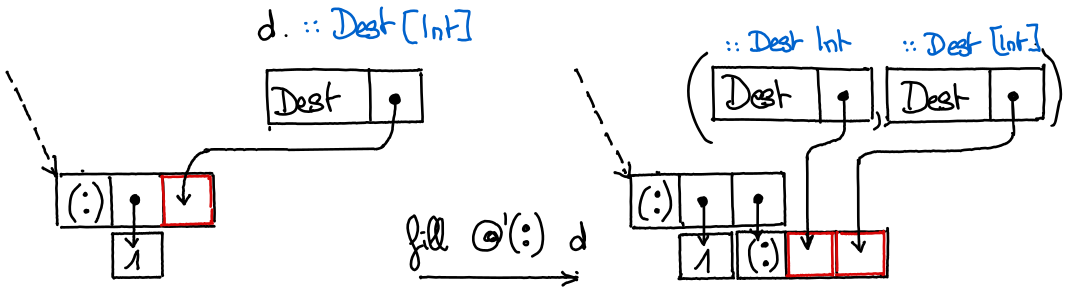
\includegraphics[width=10cm]{fillCons.png}
  \caption{Memory behavior of \mintinline{haskell}`fill @'(:) :: Dest [a] ⊸ (Dest a, Dest [a])`}
  \label{fig:schema-fillCons}
\end{figure}

\begin{figure}[t]\centering
  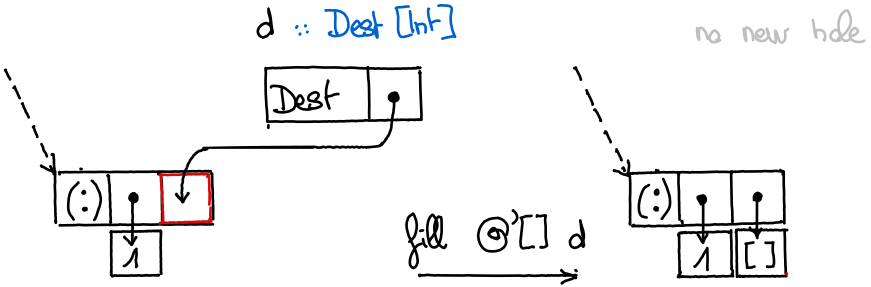
\includegraphics[width=10cm]{fillNil.png}
  \caption{Memory behavior of \mintinline{haskell}`fill @'[] :: Dest [a] ⊸ ()`}
  \label{fig:schema-fillNil}
\end{figure}

\begin{figure}[t]\centering
  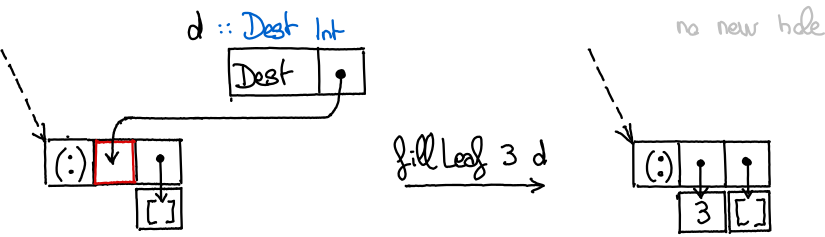
\includegraphics[width=10cm]{fillLeaf.png}
  \caption{Memory behavior of \mintinline{haskell}`fillLeaf :: a → Dest [a] ⊸ ()`}
  \label{fig:schema-fillLeaf}
\end{figure}

\begin{figure}[t]\centering
  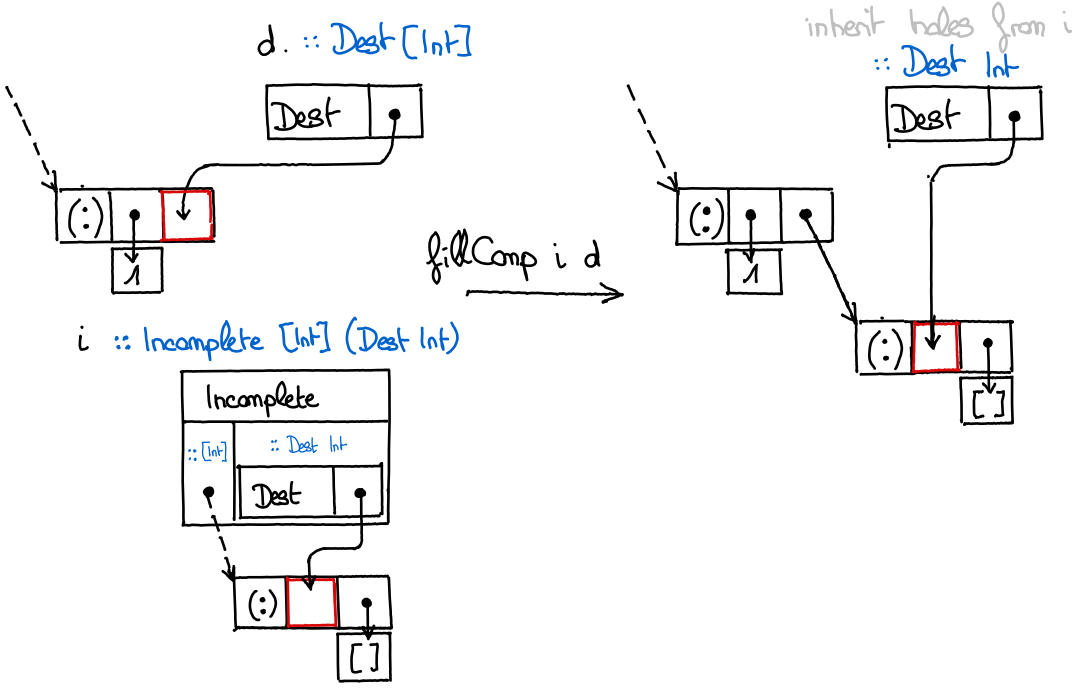
\includegraphics[width=10cm]{fillComp.png}
  \caption{Memory behavior of \mintinline{haskell}`fillComp :: Incomplete a b ⊸ Dest a ⊸ b`}
  \label{fig:schema-fillComp}
\end{figure}

\begin{figure}[t]\centering
  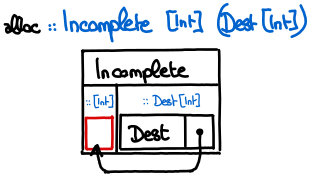
\includegraphics[width=4.2cm]{alloc.png}
  \caption{Memory behavior of \mintinline{haskell}`alloc`}
  \label{fig:schema-alloc}
\end{figure}

\begin{figure}[t]\centering
  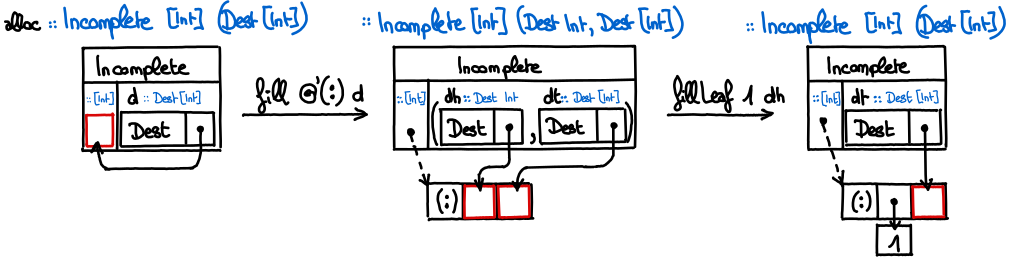
\includegraphics[width=14cm]{dlist-append.png}
  \caption{Memory behavior of \mintinline{haskell}`append alloc 1`}
  \label{fig:schema-dlist-append}
\end{figure}

\begin{figure}[t]\centering
  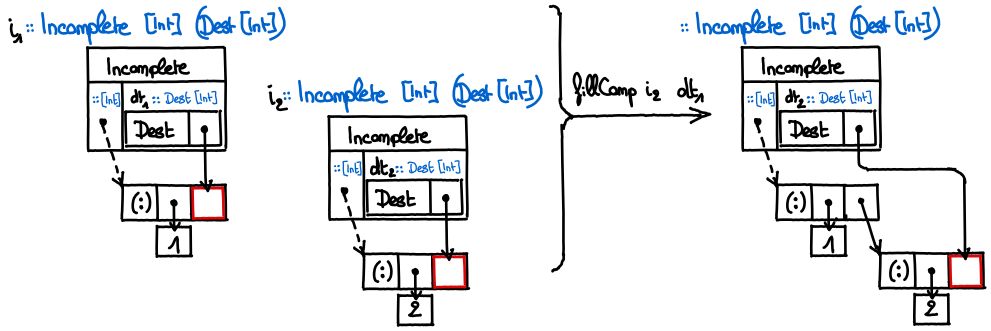
\includegraphics[width=13.5cm]{dlist-concat.png}
  \caption{Memory behavior of \mintinline{haskell}`concat i1 i2`}
  \label{fig:schema-dlist-concat}
\end{figure}

\begin{figure}[t]\centering
  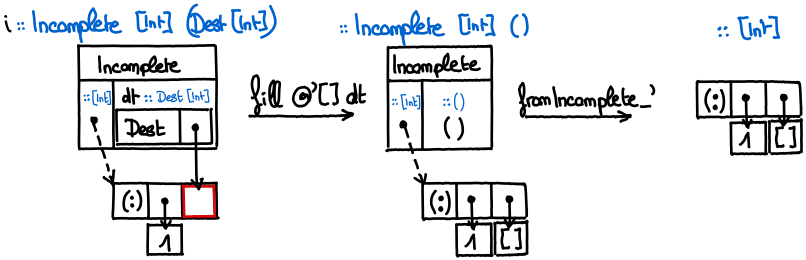
\includegraphics[width=11.5cm]{dlist-toList.png}
  \caption{Memory behavior of \mintinline{haskell}`toList i`}
  \label{fig:schema-dlist-toList}
\end{figure}

\begin{itemize}
  \item \mintinline{haskell}`alloc` returns a
    \mintinline{haskell}`DList a` which is exactly an
    \mintinline{haskell}`Incomplete [a] (Dest [a])` structure as
    depicted in Figure~\ref{fig:schema-alloc}. There is no data
    there yet and the list that will be fed in the
    \mintinline{haskell}`Dest [a]` is exactly the list that the
    resulting \mintinline{haskell}`Incomplete` will hold. This is
    highly similar to the \mintinline{haskell}`id` function which
    represents the empty destination list in the function encoding;
    

  \item \mintinline{haskell}`append` adds an element at the tail
    position of a difference list. For this, it first uses
    \mintinline{haskell}`fill @'(:)` (whose individual behavior is presented in figure~\ref{fig:schema-fillCons}) to fill the hole at the end of the list represented by 
    \mintinline{haskell}`d :: Dest [a]` with a new hollow \emph{cons}
    cell with two new holes pointed by \mintinline{haskell}`(dh :: Dest a, dt :: Dest [a])`, as illustrated in figure~\ref{fig:schema-dlist-append}. Then,
    \mintinline{haskell}`fillLeaf` (whose individual behavior is presented in figure~\ref{fig:schema-fillLeaf}) fills the hole represented by
    \mintinline{haskell}`dh` with the value
    of type \mintinline{haskell}`a`
    to append. The hole of the resulting difference list is the one pointed by \mintinline{haskell}`dt :: Dest [a]` which hasn't been filled yet.

  \item \mintinline{haskell}`concat` concates two difference lists,
    \mintinline{haskell}`i1` and list \mintinline{haskell}`i2`, by
    using \mintinline{haskell}`fillComp` (whose individual behavior is presented in figure~\ref{fig:schema-fillComp}) to fill the destination \mintinline{haskell}`dt1`
    of the first difference list \mintinline{haskell}`i1` with the
    root of the second difference list\mintinline{haskell}`i2`. The resulting \mintinline{haskell}`Incomplete`
    object hence has the same root as the first list, holds the
    elements of both lists, and inherits the hole of the second list as shown in figure~\ref{fig:schema-dlist-concat}. Memory-wise,
    \mintinline{haskell}`concat` just writes the address of the root
    of the second list into the hole of the first one; no move is
    required.

  \item \mintinline{haskell}`toList` completes the incomplete structure by plugging \emph{nil} into its hole with \mintinline{haskell}`fill @'[]` (whose individual behavior is presented in figure~\ref{fig:schema-fillNil}) and removes the \mintinline{haskell}`Incomplete` wrapper which is no longer mandatory as the structure is now complete. An overview of the whole operation is presented in figure~\ref{fig:schema-dlist-toList}.
\end{itemize}

This simplified API for difference lists still lacks some linearity requirements to make it write-once/immutable. In particular, the result of \mintinline{haskell}`alloc` should be used linearly but this isn't enforced by this API, and as a result, one could fill the embedded destination twice. Linearity concerns will be addressed in section~\ref{ssec:api-linearity}.

Thanks to destinations, we can write functions whose implementation is closer to their intended memory behavior (here, implementing data structures with holes), and get comparable or sometimes better performance than the implementations based on pure functional techniques. A performance report is available in subsection~\ref{ssec:benchmark-dlist}.

\subsection{Breadth-first tree traversal}\label{ssec:bf-tree-traversal}

Consider the problem, which Okasaki attributes to Launchbury~\cite{okasaki_bfs_2000}
\begin{quote}
  Given a tree $T$ , create a new tree of the same
  shape, but with the values at the nodes replaced
  by the numbers $1\ldots|T|$ in breadth-first order.
\end{quote}

This problem admits a straightforward implementation if we're allowed to mutate trees. But a pure implementation is quite tricky: it's the entire subject of Okasaki's paper~\cite{okasaki_bfs_2000} as well as the earlier~\cite{jones_gibbons_linearbfs_93}. More recently, a very elegant, albeit very clever, solution was proposed in~\cite{gibbons_phases_2023}.

With destinations as first-class objects in our toolbelt, we can implement a solution that is both easy to come up with and efficient, doing only a single traversal pass on the original tree. The main idea is to keep a queue of pairs of a tree to be relabeled and the destination where the the relabeled result is expected (as destinations can be stored in arbitrary containers!). DPS programming make it possible to leave some parts of the tree ``unfinished'' for some time, and to come back to them later when it's their turn to be processed, as in an imperative implementation. The implementation provided in table~\ref{table:impl-bfs-tree-traversal}, really implements the slightly more general \mintinline{haskell}`mapAccumBFS`, which traverses a tree in breadth-first order and applies a relabeling function that can depend on a state.

\begin{table}[t]
\small
\begin{minted}[linenos]{haskell}
data Tree a = Nil | Node a (Tree a) (Tree a)

relabelDPS :: Tree a → Tree Int
relabelDPS tree = fst (mapAccumBFS (\s _ → (s + 1, s)) 1 tree)

mapAccumBFS :: ∀ a b s. (s → a → (s, b)) → s → Tree a → (Tree b, s)
mapAccumBFS f s0 tree =
  fromIncomplete' (
    alloc <&> \dtree → go s0 (singleton (Ur tree, dtree)))
  where
    go :: s → Queue (Ur (Tree a), Dest (Tree b)) ⊸ Ur s
    go s q = case dequeue q of
      Nothing → Ur s
      Just ((utree, dtree), q') → case utree of
        Ur Nil → fill @'Nil dtree ;; go s q'
        Ur (Node x tl tr) → case fill @'Node dtree of
          (dr, dtl, dtr) →
            let q'' = q' `enqueue` (Ur tl, dtl) `enqueue` (Ur tr, dtr)
                (s', r) = f s x
              in fillLeaf r dr ;; go s' q''
\end{minted}
\caption{Implementation of breadth-first tree traversal with destinations}
\label{table:impl-bfs-tree-traversal}
\end{table}

Note that the signature of \mintinline{haskell}`mapAccumBFS` and \mintinline{haskell}`relabelDPS` don't involve linear types. Linear types only appear in the inner loop \mintinline{haskell}`go`, which manipulates destinations. Linearity enforces the fact that every destination ever put in the queue is eventually filled at some point, which guarantees that the output tree is complete after the function has run, and thus can be made readable.

Because the state-transforming function \mintinline{haskell}`s → a → (s, b)` is non-linear, the leaves of the original tree (that are stored together with destinations in the queue) won't be consumed in a linear fashion. However, as we said, destinations must be all consumed linearly, and for that to hold, the container they are put in must be consumed linearly too. So we wrap the input tree in \mintinline{haskell}`Ur`. As detailed in subsection~\ref{ssec:intro-linearity}, thanks to \mintinline{haskell}`Ur`, queue pairs will appeared to be consumed linearly even though the input tree leaves aren't.

With this example, we show how destinations can be used even in a non-linear setting in order to improve the expressiveness of the base language. This more natural and less convoluted implementation of breadth-first traversal also presents great performance gains compared to the fancy functional implementation from~\cite{gibbons_phases_2023}, as detailed in subsection~\ref{ssec:benchmark-bf-tree-traversal}.

\subsection{Deserializing, lifetime, and garbage collection}\label{ssec:parser-sexpr}

In client-server applications, the following pattern is very frequent: the server receives a request from a client with a serialized payload, the server then deserializes the payload, runs some code, and respond to the request. Most often, the deserialized payload is kept alive for the entirety of the request handling. In a garbage collected language, there's a real cost to this: for the entire duration of the request, the garbage collector (GC) will traverse the deserialized payload again and again. We know that, in fact, the GC doesn't need to follow all these internal pointers, because the lifetimes of the heap objects in the payload are highly correlated: they are either all live or all dead.

Instead, we'd rather consider the deserialized payload as a single heap object, which doesn't need to be traversed, and is freed as a block. GHC supports this use-case with a feature named \emph{compact regions}~\cite{yang_efficient_2015}. Compact regions contain normal heap objects, but the GC never follows pointers into a compact region. The flipside is that a compact region can only be collected when all of the objects it contains are dead.

The main API function for compact region is \mintinline{haskell}`compact :: a → Compact a`, which takes an arbitrary value and copies it in a compact region, returning a wrapper which contains both the newly-copied object and some region info. This wrapper can be discarded with \mintinline{haskell}`getCompact :: Compact a → a`. For our use-case, we can have

{\small
\begin{minted}{haskell}
let deserializedPayload = getCompact (compact (deserialize payload))
\end{minted}
}

Then the internal pointers of \mintinline{haskell}`deserializedPayload` will indeed never be followed by the GC, and the entirety of \mintinline{haskell}`deserializedPayload` will be collected at the same time.

However, we are allocating two copies of the deserialized payload: one in the regular GC heap, and one in the compact region. This is wasteful, it would be much better to be able to allocate directly in the compact region. It can be done with destinations.

In fact, as I'll explain in section~\ref{sec:implementation}, my current implementation of DPS in Haskell is backed by compact regions. Compact regions are convenient because they provide more freedom to do low-level memory operations without interfering with the GC.

Let's see how a simple parser for S-expressions can be transformed into one using destinations for greater performance. S-expressions are parenthesized lists whose elements are just separated by spaces. These elements can be of several types: int, string, symbol (a textual token, with no quotes around it, unlike a string), or a list of other S-expressions.

Parsing a S-expression can be done concisely with three mutually recursive functions:
\begin{itemize}
  \item \mintinline{haskell}`parseSExpr` scans the next character, and either dispatches to \mintinline{haskell}`parseSList` if it encounters an opening parenthesis, or to \mintinline{haskell}`parseSString` if it encounters an opening quote, or eventually parses the string into a number or symbol;
  \item \mintinline{haskell}`parseSList` calls \mintinline{haskell}`parseSExpr` to parse the next token, and then calls itself again until reaching a closing parenthesis, accumulating the parsed elements along the way;
  \item \mintinline{haskell}`parseSString` scans the input character by character and accumulates them until reaching a closing quote (taking escape sequences into consideration).
\end{itemize}

Only \mintinline{haskell}`parseSList` implementation will be presented here as it is enough for our purpose, but the full implementation of both the naive and destination-based versions can be found in tables~\ref{table:impl-sexpr-parser-without-dest} and~\ref{table:impl-sexpr-parser-with-dest}.

\begin{table}[t]
\small
\begin{minted}[linenos,escapeinside=°°]{haskell}
parseSExpr :: ByteString → Int → Either Error SExpr
parseSExpr bs i = case bs !? i of
  Nothing → Left (UnexpectedEOFSExpr i)
  Just c → case c of
    ')' → Left (UnexpectedClosingParen i)
    '(' → parseSList bs (i + 1) []
    '"' → parseSString bs (i + 1) False []
    _ → let tok = extractNextToken bs i -- take chars until delimiter/space
         in if null tok then parseSExpr bs (i + 1) else case parseInt tok of
              Just int → Right (SInteger (i + length tok - 1) int)
              Nothing → Right (SSymbol (i + length tok - 1) (toString tok))
parseSList :: ByteString → Int → [SExpr] → Either Error SExpr
parseSList bs i acc = case bs !? i of
  Nothing → Left (UnexpectedEOFSList i)
  Just c → if
    | c == ')' → Right (SList i (reverse acc))
    | isSpace c → parseSList bs (i + 1) acc
    | otherwise → case parseSExpr bs i of
        Left err → Left err
        Right child → parseSList bs (endPos child + 1) (child : acc)
parseSString :: ByteString → Int → Bool → [Char] → Either Error SExpr
parseSString bs i escape acc = case bs !? i of
  Nothing → Left (UnexpectedEOFSString i)
  Just c → case c of
    '"'  | not escape → Right (SString i (reverse acc))
    '\\' | not escape → parseSString bs (i + 1) True acc
    'n'  | escape → parseSString bs (i + 1) False ('\n' : acc)
    _ → parseSString bs (i + 1) False (c : acc)
\end{minted}
\caption{Implementation of the S-expression parser without destinations}
\label{table:impl-sexpr-parser-without-dest}
\end{table}

\begin{table}[t]
\small
\begin{minted}[linenos,escapeinside=°°]{haskell}
parseSExprDPS :: ByteString → Int → Dest SExpr ⊸ Either Error Int
parseSExprDPS bs i d = case bs !? i of
  Nothing → °\mnew{fillLeaf defaultSExpr d}° ;; Left (UnexpectedEOFSExpr i)
  Just c → case c of
    ')' → °\mnew{fillLeaf defaultSExpr d}° ;; Left (UnexpectedClosingParen i)
    '(' → parseSListDPS bs (i + 1) °\mnew{(fill @'SList d)}°
    '"' → parseSStringDPS bs (i + 1) False °\mnew{(fill @'SString d)}°
    _ → let tok = extractNextToken bs i -- take chars until delimiter/space
        in if null tok then parseSExprDPS bs (i + 1) d else case parseInt tok of
              Just int → let °\mnew{!dint = fill @'SInteger d}°
                          in °\mnew{fillLeaf int dint}° ;; Right (i + length tok - 1)
              _ → let °\mnew{!dsym = fill @'SSymbol d}°
                   in °\mnew{fillLeaf (toString tok) dsym}° ;; Right (i + length tok - 1)
parseSListDPS :: ByteString → Int → Dest [SExpr] ⊸ Either Error Int
parseSListDPS bs i d = case bs !? i of
  Nothing → °\mnew{fill @'[] d}° ;; Left (UnexpectedEOFSList i)
  Just c → if
    | c == ')' → °\mnew{fill @'[] d}° ;; Right i
    | isSpace c → parseSListDPS bs (i + 1) d
    | otherwise → let !(dh, dt) = °\mnew{fill @'(:) d}°
                   in case parseSExprDPS bs i °\mnew{dh}° of
                        Left err → fill @'[] dt ;; Left err
                        Right endPos → parseSListDPS bs (endPos + 1) °\mnew{dt}°
parseSStringDPS :: ByteString → Int → Bool → Dest [Char] ⊸ Either Error Int
parseSStringDPS bs i escape d = case bs !? i of
  Nothing → °\mnew{fill @'[] d}° ;; Left (UnexpectedEOFSString i)
  Just c → case c of
    '"'  | not escape → °\mnew{fill @'[] d}° ;; Right i
    '\\' | not escape → parseSStringDPS bs (i + 1) True d
    'n'  | escape → let °\mnew{!(dh, dt) = fill @'(:) d}°
                     in °\mnew{fillLeaf '\textbackslash{}n' dh}° ;; parseSStringDPS bs (i + 1) False °\mnew{dt}°
    _ → let °\mnew{!(dh, dt) = fill @'(:) d}°
         in °\mnew{fillLeaf c dh}° ;; parseSStringDPS bs (i + 1) False °\mnew{dt}°
\end{minted}
\caption{Implementation of the S-expression parser with destinations}
\label{table:impl-sexpr-parser-with-dest}
\end{table}

{\small
\begin{minted}[linenos]{haskell}
parseSList :: ByteString → Int → [SExpr] → Either Error SExpr
parseSList bs i acc = case bs !? i of
  Nothing → Left (UnexpectedEOFSList i)
  Just c → if
    | c == ')' → Right (SList i (reverse acc))
    | isSpace c → parseSList bs (i + 1) acc
    | otherwise → case parseSExpr bs i of
        Left err → Left err
        Right child → parseSList bs (endPos child + 1) (child : acc)
\end{minted}
}

This tail-recursive implementation above is quite standard: the accumulator \mintinline{haskell}`acc` collects the nodes that are returned by the call to \mintinline{haskell}`parseSExpr` in the reverse order (because it's the natural building order for a linked list without destinations). When the end of the SList is reached (line 5), the accumulator is reversed and stored in the \mintinline{haskell}`SList` constructor, before being returned.

We will see that destinations can bring very significative performance gains with only very little stylistic changes in the code. Accumulators of tail-recursive functions just have to be changed into destinations. Instead of writing elements into a list that will be reversed at the end as we did before, the program in the destination style will directly write the elements into their final location:

{\small
\begin{minted}[linenos,escapeinside=°°]{haskell}
parseSListDPS :: ByteString → Int → Dest [SExpr] ⊸ Either Error Int
parseSListDPS bs i d = case bs !? i of
  Nothing → °\mnew{fill @'[] d}° ;; Left (UnexpectedEOFSList i)
  Just c → if
    | c == ')' → °\mnew{fill @'[] d}° ;; Right i
    | isSpace c → parseSListDPS bs (i + 1) d
    | otherwise →
        let !(dh, dt) = °\mnew{fill @'(:) d}°
         in case parseSExprDPS bs i °\mnew{dh}° of
              Left err → fill @'[] dt ;; Left err
              Right endPos → parseSListDPS bs (endPos + 1) °\mnew{dt}°
\end{minted}
}

Let's see what changed compared to the naive implementation:

\begin{itemize}
  \item even for error cases, we are forced to consume the destination that we receive as an argument, hence we write some sensible default data to it (see line 3);
  \item the \mintinline{haskell}`SExpr` value resulting from the call of \mintinline{haskell}`parseSExprDPS` is not collected by \mintinline{haskell}`parseSListDPS`; but instead written directly into its final location by \mintinline{haskell}`parseSExprDPS` through the passing and filling of destination \mintinline{haskell}`dh` (see line 9);
  \item adding an element of type \mintinline{haskell}`SExpr` to the accumulator \mintinline{haskell}`[SExpr]` is replaced with adding a new cons cell with \mintinline{haskell}`fill @'(:)` into the hole represented by \mintinline{haskell}`Dest [SExpr]`, writing an element to the ``head'' destination, and then doing a recursive call with the ``tail'' destination passed as an argument (which has type \mintinline{haskell}`Dest [SExpr]` again);
  \item instead of reversing and returning the accumulator at the end of the processing, it is enough to complete the list by writing a nil element to the tail destination (with \mintinline{haskell}`fill @'[]`) (see line 5).
\end{itemize}

It is important to note that destinations allow to reverse the natural order in which a structure is built. For a list, the natural operation in functional programming languages is \emph{prepend}/\mintinline{haskell}`(:)`, which adds an element at the front of an existing list (bottom-up approach). Thanks to destinations, it's possible to build a list starting from an element which will stay at the head of the it, and add new elements towards the tail of the list (top-down approach, with \emph{append}/\mintinline{haskell}`fill @'(:)`). Of course, it is possible to mix both approaches, thanks to \mintinline{haskell}`fillComp`/\mintinline{haskell}`fillLeaf`.

Thanks to that new implementation which is barely longer (in terms of lines of code) than the naive one, the program runs almost twice as fast, mostly because garbage-collection time goes to almost zero. The detailed benchmark is available in section~\ref{ssec:benchmark-parser}.

\section{API Design}\label{sec:api}

\begin{table}[t]
\small
\begin{minted}[linenos]{haskell}
data Token
consume   ::      Token ⊸ ()
dup2      ::      Token ⊸ (Token, Token)
withToken :: ∀ a. (Token ⊸ Ur a) ⊸ Ur a

data Incomplete a b
fmap                :: ∀ a b c. (b ⊸ c) ⊸ Incomplete a b ⊸ Incomplete b c
alloc               :: ∀ a.     Token ⊸ Incomplete a (Dest a)
intoIncomplete      :: ∀ a.     Token ⊸ a → Incomplete a ()
fromIncomplete_     :: ∀ a.     Incomplete a () ⊸ Ur a
fromIncomplete      :: ∀ a b.   Incomplete a (Ur b) ⊸ Ur (a, b)
-- fromIncomplete_' :: ∀ a.     Incomplete a () ⊸ a
-- fromIncomplete'  :: ∀ a b.   Incomplete a (Ur b) ⊸ (a, b)

data Dest a
type family DestsOf lCtor a -- returns dests associated to fields of constructor
fill     :: ∀ lCtor a. Dest a → DestsOf lCtor a
fillComp :: ∀ a b.     Incomplete a b ⊸ Dest a ⊸ b
fillLeaf :: ∀ a.       a → Dest a ⊸ ()
\end{minted}
\caption{Destination API for Haskell}
\label{table:destination-api}
\end{table}

\subsection{The \texttt{Incomplete} type}

The main design principle behind DPS structure building is that no structure can be read before all its destinations have been filled. That way, incomplete data structures can be freely passed around and stored, but need to be completed before any pattern-matching can be made on them.

Hence we introduce a new data type \mintinline{haskell}`Incomplete a b` where \mintinline{haskell}`a` stands for the type of the structure being built, and \mintinline{haskell}`b` is the type of what needs to be linearly consumed before the structure can be read. The idea is that one can map over the \mintinline{haskell}`b` side, which will contains destinations or containers with destinations inside, until there is no destination left but just a non-linear value that can safely escape (e.g. \mintinline{haskell}`()`, an integer, or something wrapped in \mintinline{haskell}`Ur`). When destinations from the \mintinline{haskell}`b` side are consumed, the structure on the \mintinline{haskell}`a` side is built little by little in a top-down fashion, as we showed in figures~\ref{fig:schema-dlist-append} and \ref{fig:schema-dlist-concat}. And when no destination remains on the \mintinline{haskell}`b` side, the \mintinline{haskell}`a` value no longer has holes, thus is ready to be released/read.

It can be released in two ways: with \mintinline{haskell}`fromIncomplete_`, the value on the \mintinline{haskell}`b` side must be unit (\mintinline{haskell}`()`), and just the \mintinline{haskell}`a` value is returned. With \mintinline{haskell}`fromIncomplete`, the value on the \mintinline{haskell}`b` side must be of the form  \mintinline{haskell}`Ur b'`, and then the pair of type \mintinline{haskell}`(a, b')` is returned.

Because the leaves of the structure that has been built either come from non-linear sources (as \mintinline{haskell}`fillLeaf :: a → Dest a ⊸ ()` consumes its first argument non-linearly) or are made of 0-ary constructors added with \mintinline{haskell}`fill`, the whole structure can safely be used in a non-linear fashion. That's why \mintinline{haskell}`fromIncomplete_` and \mintinline{haskell}`fromIncomplete` actually wrap their result in \mintinline{haskell}`Ur`. The variants \mintinline{haskell}`fromIncomplete_'` and \mintinline{haskell}`fromIncomplete'` that have been used in the beginning of this article just drop the \mintinline{haskell}`Ur` wrapper.

The function \mintinline{haskell}`toIncomplete` takes a non-linear argument of type \mintinline{haskell}`a` and wraps it into an already-complete \mintinline{haskell}`Incomplete` with no destination on the \mintinline{haskell}`b` side. \mintinline{haskell}`fromIncomplete_' . toIncomplete token` and \mintinline{haskell}`toIncomplete token . fromIncomplete_'` might do a few unnecessary allocations, but are both equivalent to the identity function.

The whole API is presented in table~\ref{table:destination-api}.

\subsection{Ensuring write-once model for holes with linear types}\label{ssec:api-linearity}

\TODO{Linear constraints paper?}\cite{spiwack_linearly_2022}

Types aren't linear by themselves in Linear Haskell. Instead, functions can be made linear or not, but that's all. So in direct style --- where consumers of a resource are implicit/not know yet by the producer --- there is no way to state that a specific resource must be used exactly once:

{\small
\begin{minted}[linenos]{haskell}
createR :: () ⊸ Resource -- no way to indicate that the result must be used once
consumeR :: Resource ⊸ ()

exampleShouldFail :: ()
exampleShouldFail =
  let r :: Resource = createR ()
   in consumeR r ;; consumeR r -- OK even though the resource r is consumed twice
\end{minted}
}

The solution is to make the production of the resource implicit but force the consumers to become explicit and check their signature:

{\small
\begin{minted}[linenos,escapeinside=°°]{haskell}
withR :: (Resource ⊸ a) ⊸ a
consumeR :: Resource ⊸ ()

exampleFail :: ()
exampleFail = withR (\r → consumeR °\mold{r}° ;; consumeR °\mold{r}°) -- the callback isn't linear
\end{minted}
}

The \mintinline{haskell}`Resource` type is in positive position in the signature of \mintinline{haskell}`withR`, so that function should somehow know how to produce a \mintinline{haskell}`Resource`, but this is opaque for the user. Because the consumer of the resource must now be explicitly passed to \mintinline{haskell}`withR`, and is a function, the signature of \mintinline{haskell}`withR` can enforce that every consumer must be a linear function that will use the resource exactly once.

Still, this is not enough; because \mintinline{haskell}`\x → x` is indeed a linear callback, one could use \mintinline{haskell}`withR (\x → x)` to leak a \mintinline{haskell}`Resource`, and then use it in a non-linear fashion in the outside world. Hence we must forbid the resource from appearing anywhere in the return type of the callback. To do that, we will ask the return type to be wrapped in \mintinline{haskell}`Ur`: because the resource comes from the left of a linear arrow, and doesn't implement \mintinline{haskell}`Movable`, it cannot be wrapped in \mintinline{haskell}`Ur` without breaking linearity, so won't be able to escape (see subsection~\ref{ssec:intro-linearity}). But a \mintinline{haskell}`Movable` value of type \mintinline{haskell}`()` or \mintinline{haskell}`Int` can be returned:
{\small
\begin{minted}[linenos,escapeinside=°°]{haskell}
withR' :: (Resource ⊸ Ur a) ⊸ Ur a
consumeR :: Resource ⊸ ()

exampleOk' :: Ur ()
exampleOk' = withR' (\r → let u :: () = consumeR r' in move u)
exampleFail' :: Ur Resource
exampleFail' = withR' (\r → °\mold{Ur r}°) -- the callback isn't linear
\end{minted}
}

This is exactly the principle that have been used for the DPS implementation in Haskell. \mintinline{haskell}`Incomplete a b` has a \mintinline{haskell}`Control.Functor.Linear` instance to map on the \mintinline{haskell}`b` side --- the one carrying destinations --- which forces the callback to be linear:

{\small
\begin{minted}[escapeinside=°°]{haskell}
instance Control.Functor.Linear (Incomplete a) where
  fmap :: ∀ b c. (b ⊸ c) ⊸ Incomplete a b ⊸ Incomplete b c
  fmap f (Incomplete (s, d)) = Incomplete (s, f d)
\end{minted}
}

And \mintinline{haskell}`alloc :: ∀ a. Token ⊸ Incomplete a (Dest a)` is the only function in which a \mintinline{haskell}`Dest` appears in positive position, but locked by an \mintinline{haskell}`Incomplete` (which is an opaque wrapper for the user). So destinations can only ever be accessed by mapping over an \mintinline{haskell}`Incomplete` with \mintinline{haskell}`fmap`, and cannot leak to the outside. It isn't possible either for a \mintinline{haskell}`Dest a` to be linearly consumed by filling another \mintinline{haskell}`Dest (Dest a)` with \mintinline{haskell}`fillLeaf`, as the first argument of the \mintinline{haskell}`fillLeaf` function isn't used linearly.\footnote{It would actually be desirable to have \mintinline{haskell}`Dest (Dest a)` work. But it turns out that doing so naively compromises the type safety properties related to linearity that we describe in this section. How to recover type safety in presence of destinations of destinations is still an open problem.}

Morally, this linear \mintinline{haskell}`Functor` instance says that one can temporary forget about the root of the structure under construction, and just manipulate the destinations as first-class objects that will produce remote building effects onto the structure that is invisible in the inner scope.

\paragraph{Ensuring linear use of \texttt{Incomplete} objects}

We made sure that destinations inside \mintinline{haskell}`Incomplete` objects could only be used linearly, and now we need to do the same for \mintinline{haskell}`Incomplete`s themselves. For that, we introduce a new token type \mintinline{haskell}`Token`. A token can be linearly exchanged one for one with an \mintinline{haskell}`Incomplete` of any type through \mintinline{haskell}`alloc`, and can be linearly duplicated with \mintinline{haskell}`dup2` or linearly deleted with \mintinline{haskell}`consume`. However, it cannot be linearly stored in \mintinline{haskell}`Ur` as it doesn't implement \mintinline{haskell}`Movable`.

As in the example above, we just ensure that \mintinline{haskell}`withToken :: ∀ a. (Token ⊸ Ur a) ⊸ Ur a` is the only source of \mintinline{haskell}`Token`s around. Now, to produce an \mintinline{haskell}`Incomplete` with \mintinline{haskell}`alloc`, one must get a token first, so has to be in the scope of a callback which is passed to \mintinline{haskell}`withToken`. Putting either a \mintinline{haskell}`Token` or \mintinline{haskell}`Incomplete` in \mintinline{haskell}`Ur` inside the callback would then make the callback non-linear. So none of them can escape the scope as is, but a structure built from an \mintinline{haskell}`Incomplete` and finalized with \mintinline{haskell}`fromIncomplete` or \mintinline{haskell}`fromIncomplete_` would be automatically wrapped in \mintinline{haskell}`Ur`, and could safely escape the scope\footnote{This is why \mintinline{haskell}`fromIncomplete'` and \mintinline{haskell}`fromIncomplete_'` aren't that useful in the memory-safe API: the built structure would be stuck in the scope function without its \mintinline{haskell}`Ur` free pass around.}.

\subsection{Filling functions for destinations}

The last part of the API is the one in charge of actually building the structures in a top-down fashion, using layers of hollow constructors. 

To fill a hole represented by \mintinline{haskell}`Dest a`, three functions are available:

\paragraph{\texttt{fillLeaf} function}

\mintinline{haskell}`fillLeaf :: ∀ a. a → Dest a ⊸ ()` will use a value of type \mintinline{haskell}`a` to fill the hole represented by the destination. The destination is consumed linearly, but the value to fill the hole isn't (as indicated by the first non-linear arrow). Memory-wise, the address of the object \mintinline{haskell}`a` is written into the memory cell whose address is carried by the destination (see figure~\ref{fig:schema-fillLeaf}).

\paragraph{\texttt{fillComp} function}

\mintinline{haskell}`fillComp :: ∀ a b. Incomplete a b ⊸ Dest a ⊸ b` is used to plug two \mintinline{haskell}`Incomplete` objects together. The parent \mintinline{haskell}`Incomplete` object into which the child \mintinline{haskell}`Incomplete` will be plugged isn't represented in the signature of the function. Instead, only the hole of the parent that will host the address of the child is represented by the \mintinline{haskell}`Dest a`; and \mintinline{haskell}`Incomplete a b` in the signature refers to the child object. A call to \mintinline{haskell}`fillComp` always takes place in the scope of \mintinline{haskell}`fmap` over the parent object (or \mintinline{haskell}`<&>` which is \mintinline{haskell}`fmap` with the order of the arguments reversed):
{\small
\begin{minted}[linenos,escapeinside=°°]{haskell}
parent :: Incomplete BigStruct (Dest SmallStruct, Dest OtherStruct)
child :: Incomplete SmallStruct (Dest Int)

comp = parent <&> \(ds, extra) → fillComp child ds
       :: Incomplete BigStruct (Dest Int, Dest OtherStruct)
\end{minted}
}
The resulting structure \mintinline{haskell}`comp` is morally a \mintinline{haskell}`BigStruct`, that inherited the holes from the child structure (represented by the \mintinline{haskell}`Dest Int`). The other destination from the parent, \mintinline{haskell}`Dest OtherStruct`, is still there to be filled. The memory behavior of \mintinline{haskell}`fillComp` can be seen in figure~\ref{fig:schema-fillComp}.

\paragraph{\texttt{fill} function}

\mintinline{haskell}`fill` is probably the most interesting of the three, and will be the most used one too, because it enables the user to build data structures in a top-down approach, which complements very well the natural bottom-up way of constructing data structures in functional programming languages. Thanks to DPS programming for Haskell, the user can now choose between those two approaches and pick the most efficient or more natural way for the problem at hand.

The concept of \mintinline{haskell}`fill :: ∀ lCtor a. Dest a ⊸ DestsOf lCtor a` is to take a constructor as a type parameter (\mintinline{haskell}`lCtor`) and to allocate a hollow heap object that has the same header/tag as the specified constructor but unspecified fields. The address of the allocated hollow constructor is written in the destination that is passed to \mintinline{haskell}`fill`. As a result, one hole is now filled, but there is one new hole in the structure for each field left unspecified in the hollow constructor that is now part of the bigger structure. So \mintinline{haskell}`fill` returns one destination of matching type for each of the fields of the constructor. The memory behavior of \mintinline{haskell}`fill @'(:) :: Dest [a] ⊸ (Dest a, Dest [a])` is given in figure~\ref{fig:schema-fillCons} and the one of \mintinline{haskell}`fill @'[] :: Dest [a] ⊸ ()` is given in figure~\ref{fig:schema-fillNil}.

\mintinline{haskell}`DestsOf` is a type family (i.e. a function operating on types and returning a type) whose role is to map a constructor to the type of destinations for its fields. For example, \mintinline{haskell}`DestsOf 'Nil [a] = ()`, \mintinline{haskell}`DestsOf '(:) [a] = (Dest a, Dest [a])`, and \mintinline{haskell}`DestsOf 'Ur (Ur a) = Dest a`. There is hence a duality between the type of a constructor \mintinline[escapeinside=°°]{haskell}`C :: (f°$_i$°)°$_{i \in 1..n}$° → a` and the associated destination-filling function \mintinline[escapeinside=°°]{haskell}`fill @'C :: Dest a ⊸ (Dest f°$_i$°)°$_{i \in 1..n}$°`: the side of the arrow on which types resides is flipped, and a \mintinline{haskell}`Dest` prefix is added to each of them. Destination-based data building can be seen as more general than the usual bottom-up constructor approach, as it is possible to emulate the signature and behavior of a given constructor \mintinline{haskell}`C` with DPS programming, as shown in table~\ref{table:emulate-ctor}, whereas all the advantages of DPS programming that we described in section~\ref{sec:motivating-examples} cannot be emulated by the use of constructors alone.

\begin{table}[t]
\small
\begin{minted}[linenos,escapeinside=°°]{haskell}
C :: (f°$_i$°)°$_{i \in 1..n}$° → a

C' :: (f°$_i$°)°$_{i \in 1..n}$° → a
C' (x°$_i$°)°$_{i \in 1..n}$° = fromIncomplete_' (
  alloc <&> \(d :: Dest a) → case fill @'C d of
    (dx°$_i$°)°$_{i \in 1..n}$° → ;;°$_{i \in 1..n}$° (fillLeaf x°$_i$° dx°$_i$°))
\end{minted}
\caption{Emulating a constructor \texttt{C} with the destination-filling function \texttt{fill @'C}}
\label{table:emulate-ctor}
\end{table}

\section{Implementing destinations in Haskell}\label{sec:implementation}

Having incomplete memory structures in memory inherently introduces a lot of tension with both the garbage collector and compiler. Indeed, the GC assumes that every heap object it traverses is well-formed, whereas incomplete structures are absolutely ill-formed: they contain uninitialized pointers, which the GC should absolutely not follow.

The tension with the compiler is of lesser extent. The latter can make some optimizations because it assumes that every object is immutable, while DPS programming break that guarantee by mutating constructors after they have been allocated (albeit only one update can happen). Fortunately, most if not all of those errors can be detected when implementing the API and are easily fixed with careful use of pragmas.

\subsection{Compact Regions}\label{ssec:impl-compact-regions}

As we teased in subsection~\ref{ssec:parser-sexpr}, \emph{compact regions} from~\cite{yang_efficient_2015} make it very convenient to implement DPS programming in 
Haskell. A compact region represents a memory area in the Haskell heap, that is almost fully independent from the GC and the rest of the garbage-collected heap. For the GC, each compact region is seen as a single heap object with a single lifetime. The GC can efficiently check whether there is at least one pointer in the garbage-collected heap that points into the region, and while that is the case, the region is kept alive. When this condition is no longer matched, the whole region is discarded.

The result is that the GC won't traverse any node from the region: it is treated as one opaque block. In reality, a compact region is made of several blocks of the same size, so that it can grow efficiently when needed, but that doesn't change how things operate at a higher level. Also, compact regions are immobile in memory; the GC doesn't have to and won't move them.

Hence, using compact regions to implement destinations, we completely elude the concerns of tension between the garbage collector and incomplete structures we want to build. That is also why Haskell is a good candidate to experiment with DPS programming in an immutable, functional context: it has support for both linear types and compact regions; the former is used to make the interface safe, the latter to make the implementation safe.

There are only two restrictions associated to compact regions. Firstly, every structure in a region must be in a fully-evaluated form. Regions are strict, and any piece of data that is copied to a region is first forced into normal form. This might not be a win for every use-case; sometimes laziness -- which is the default \emph{modus operandi} of the garbage-collected heap --- might be preferable.

Secondly, data in a region cannot contain pointers to the garbage-collected heap, or pointers to other regions: it must be self-contained. That forces us to slightly modify the API, to add a phantom type parameter \mintinline{haskell}`r` which tags each object with the identifier of the region it belongs to. A typeclass \mintinline{haskell}`Region r` is also needed to carry around the details about a region that are required in the implementation of the API functions. The API for DPS programming backed by compact regions is available in table~\ref{table:destination-api-regions} (The \mintinline{haskell}`Token` type and its associated functions \mintinline{haskell}`dup2` and \mintinline{haskell}`consume` are unchanged).

The forced isolation of each region has a two main consequences:
\begin{itemize}
  \item \mintinline{haskell}`fillLeaf` has to copy each ``leaf'' value from the garbage-collected heap into the region in which it will be used as a leaf;
  \item \mintinline{haskell}`fillComp` can only plug together two incomplete structures that originate from the same region.
\end{itemize}

\begin{table}[t]
\small
\begin{minted}[linenos,escapeinside=°°]{haskell}
type Region r :: Constraint
°\mnew{withRegion :: ∀ a. (∀ r. Region r ⇒ Token ⊸ Ur a) ⊸ Ur a}°

data Incomplete r a b
fmap            :: ∀ r a b c. (b ⊸ c) ⊸ Incomplete r a b ⊸ Incomplete r b c
alloc           :: ∀ r a.     Region r ⇒ Token ⊸ Incomplete r a (Dest r a)
intoIncomplete  :: ∀ r a.     Region r ⇒ Token ⊸ a → Incomplete r a ()
fromIncomplete_ :: ∀ r a.     Region r ⇒ Incomplete r a () ⊸ Ur a
fromIncomplete  :: ∀ r a b.   Region r ⇒ Incomplete r a (Ur b) ⊸ Ur (a, b)

data Dest r a
type family DestsOf lCtor r a
fill     :: ∀ lCtor r a. Region r ⇒ Dest r a → DestsOf lCtor r a
fillComp :: ∀ r a b.     Region r ⇒ Incomplete r a b ⊸ Dest r a ⊸ b
fillLeaf :: ∀ r a.       Region r ⇒ a → Dest r a ⊸ ()
\end{minted}
\caption{Destination API using compact regions}
\label{table:destination-api-regions}
\end{table}

As we now have immobile chunks of memory, destinations can be implemented as a wrapper over a raw pointer (type \mintinline{haskell}`Addr#`) which points to the memory location where data have to be written:

{\small
\begin{minted}{haskell}
data Dest r a = Dest Addr#
\end{minted}
}

The \mintinline{haskell}`Region r` typeclass has a single method \mintinline{haskell}`reflect`, not available to the user, that returns the \mintinline{haskell}`RegionInfo` structure associated to identifier \mintinline{haskell}`r`. We use the \mintinline{haskell}`reflection` library (providing \mintinline{haskell}`Data.Reflection`) to make that possible.

The \mintinline{haskell}`withRegion` function is the new addition to the API. It is mostly a refinement over the \mintinline{haskell}`withToken` function from table~\ref{table:destination-api}. It receives a callback that must be agnostic in \mintinline{haskell}`r` (i.e. in which \mintinline{haskell}`r` must be a free type variable). It then spawns both a new compact region and a fresh type \mintinline[escapeinside=°°]{haskell}`°\muline{r}°` (not a variable), and then uses \mintinline{haskell}`Data.Reflection.reify` to provide an instance of \mintinline[escapeinside=°°]{haskell}`Region °\muline{r}°` on-the-fly that links \mintinline[escapeinside=°°]{haskell}`°\muline{r}°` and the \mintinline{haskell}`RegionInfo` for the newly spawned region, and calls the callback with \mintinline{haskell}`r` instantiated to \mintinline[escapeinside=°°]{haskell}`°\muline{r}°`.

\subsection{Representation of \texttt{Incomplete} objects}

Ideally, as we detailed in the API, we want \mintinline{haskell}`Incomplete r a b` to contains a \mintinline{haskell}`a` and a \mintinline{haskell}`b`, and let the \mintinline{haskell}`a` free when the \mintinline{haskell}`b` is fully consumed (or linearly transformed into \mintinline{haskell}`Ur c`). So the most straightforward memory representation of an \mintinline{haskell}`Incomplete r a b` would be a pair of an (incomplete) \mintinline{haskell}`a` and a \mintinline{haskell}`b`.

It is also natural for \mintinline{haskell}`alloc` to return an \mintinline{haskell}`Incomplete r a (Dest a)`: it represents a (future) structure of type \mintinline{haskell}`a` with a hole of type \mintinline{haskell}`a`. It's a bit like the identity function: there is nothing more here than an empty memory cell (named named \emph{root receiver}) which the associated destination points to, as presented in figure~\ref{fig:schema-alloc}.

If \mintinline{haskell}`Incomplete r a b` is represented by a pair \mintinline{haskell}`(a, b)`, then the root receiver should be the first field of the pair. But the \mintinline{haskell}`Incomplete` object shouldn't be part of the compact region itself, whereas the root of the structure under construction, that will eventually live inside the root receiver, must be in the region (because of the risk of the GC following garbage pointers). Indeed, we want the \mintinline{haskell}`Incomplete` wrapper to be optimized away by the compiler when possible, and to be deallocated as soon as possible, both of which aren't possible if it lives in the region.

One potential solution is to represent \mintinline{haskell}`Incomplete r a b` by a pair \mintinline{haskell}`(Ur a, b)`. The \mintinline{haskell}`Ur` wrapper is allocated inside the region, and its field of type \mintinline{haskell}`a` is the root receiver. With that approach, the issue of \mintinline{haskell}`alloc`'s result representation is solved, but every \mintinline{haskell}`Incomplete` wrapper will now allocate a few words in the region (to host the \mintinline{haskell}`Ur` hollow constructor) that won't be collected by the GC until a long time. This makes \mintinline{haskell}`intoIncomplete` quite inefficient memory-wise too, as the \mintinline{haskell}`Ur` wrapper is only useful for actual incomplete structures, but useless for already complete ones.

The desired outcome is to only allocate a root receiver in the region for actual incomplete structures, and skip that allocation for already complete structures that are turned into an \mintinline{haskell}`Incomplete` object, while preserving a same type for both use-cases. This is made possible by replacing the \mintinline{haskell}`Ur` wrapper inside the \mintinline{haskell}`Incomplete` by an 
indirection object (\mintinline{haskell}`stg_IND` symbol) for the actually-incomplete case. \mintinline{haskell}`Incomplete r a b` will be represented by a pair \mintinline{haskell}`(a, b)` allocated in the garbage-collected heap, but:
\begin{itemize}
  \item in the pair \mintinline{haskell}`(a, b)` returned by \mintinline{haskell}`alloc`, the \mintinline{haskell}`a` side points to an indirection object (a sort of constructor with one field, whose resulting type \mintinline{haskell}`a` is the same as the field type \mintinline{haskell}`a`), that is allocated in the region, and serve as the root receiver;
  \item in the pair \mintinline{haskell}`(a, b)` returned by \mintinline{haskell}`intoIncomplete`, the \mintinline{haskell}`a` side directly points to the object of type \mintinline{haskell}`a` that has been copied to the region.
\end{itemize}

\begin{figure}[t]\centering
  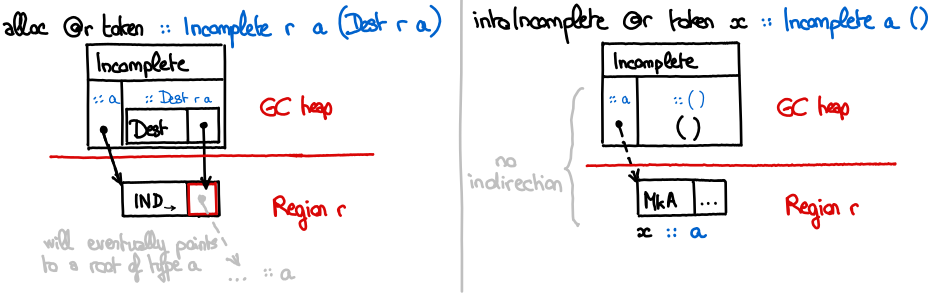
\includegraphics[width=12cm]{alloc-region.png}
  \caption{Memory behaviour of \mintinline{haskell}`alloc` and \mintinline{haskell}`intoIncomplete` in the compact region implementation}
  \label{fig:schema-alloc-region}
\end{figure}

This behavior is illustrated in figure~\ref{fig:schema-alloc-region}.

The implementation of \mintinline{haskell}`fromIncomplete` and \mintinline{haskell}`fromIncomplete_` is then relatively straightforward. They allocate a hollow \mintinline{haskell}`Ur _` or \mintinline{haskell}`Ur (_, _)` in the region, writes the address of the now complete structure into it, and returns the \mintinline{haskell}`Ur`.

\subsection{Deriving \texttt{fill} for all constructors with \texttt{Generics}}\label{ssec:impl-generics}

As it has been said before, the action of \mintinline{haskell}`fill @lCtor @r @a` is to plug a new hollow constructor \mintinline{haskell}`Ctor _ :: a` into the hole of an existing incomplete structure, and return one destination object per new hole in the structure (corresponding to the unspecified fields of the new hollow constructor).

Naively, we would need one \mintinline{haskell}`fill` function per constructor, but that cannot be realistically implemented. Instead, we have to generalize all \mintinline{haskell}`fill` functions into a typeclass, and derive an instance of the typeclass (i.e. implement \mintinline{haskell}`fill`) generically for any constructor, based only on statically-known information about that constructor.

So we need to know how to:
\begin{enumerate}
  \item allocate the actual hollow heap object for the specified constructor. That will be addressed in subsection~\ref{ssec:impl-ghc}, so let's consider for now that we have the required primitives;
  \item write the address of the new heap object at the address carried by the destination passed as an argument to \mintinline{haskell}`fill`. This is easily dealt with using memory primitives given by GHC such as \mintinline{haskell}`writeAddrOffAddr#`;
  \item find the number of holes in the new heap object, compute their adresses, and return them as destinations;
  \item give a generalized return type to the \mintinline{haskell}`fill` function that the type system can understand.
\end{enumerate}

So only points 3 and 4 remains, for which we basically need to know what are the fields of a given constructor at compile time. If we know their number, we can compute their addresses easily, as fields of a constructor are stored contiguously in memory, where the $i$\textsuperscript{th} field is stored at offset $i \times wordsize$ from the constructor base address\footnote{The exception to this layout rule are unboxed or inlined fields, which are not represented by a pointer of fixed size in the parent object. Instead, they are wholly contained in the parent object, and can span over a couple of words. At the moment, constructors with inlined or unboxed fields are not supported by \mintinline{haskell}`fill`. For such a constructor, one has to allocate the constructor in the garbage-collected heap in the normal way and then use \mintinline{haskell}`fillLeaf` or \mintinline{haskell}`toIncomplete` to incorporate it into an \mintinline{haskell}`Incomplete` structure.}. If we know their types at compile time, we can compute the return type of \mintinline{haskell}`fill`: just prefix each of them with \mintinline{haskell}`Dest r` and put them in a tuple, \emph{et voilà}!

So we will leverage \mintinline{haskell}`GHC.Generics` to find the required information. \mintinline{haskell}`GHC.Generics` is a built-in Haskell library that provides compile-time inspection of a type metadata through the \mintinline{haskell}`Generic` typeclass: list of constructors, fields, memory representation, etc. And that typeclass can be derived automatically for any type! Here's, for example, the \mintinline{haskell}`Generic` representation of \mintinline{haskell}`Maybe a`:

{\small
\begin{minted}[linenos,escapeinside=°°]{haskell}
repl> :k! Rep (Maybe a) () -- display the Generic representation of Maybe a
M1 D (MetaData "Maybe" "GHC.Maybe" "base" False) (
  M1 C (MetaCons "Nothing" PrefixI False) U1
  :+: M1 C (MetaCons "Just" PrefixI False) (M1 S [...] (K1 R a)))
\end{minted}
}

We see that there are two different possible constructors (indicated by lines starting with \mintinline{haskell}`M1 C`): the first one, \mintinline{haskell}`Nothing`, has zero field (indicated by \mintinline{haskell}`U1`), and the second one, \mintinline{haskell}`Just`, has one field of type \mintinline{haskell}`a` (indicated by \mintinline{haskell}`K1 R a`).

Back to our API, we introduce a type family (a function from type to type) \mintinline{haskell}`DestsOf (lCtor :: k) (a :: Type) :: Type` that inspects the \mintinline{haskell}`Generic` representation of a given type \mintinline{haskell}`a` in search of the chosen constructor \mintinline{haskell}`lCtor`, extracts the number and type of its fields, and return the tuple type where all the fields types are prefixed by \mintinline{haskell}`Dest r`. That's it, we now have a proper way to talk about the return type of \mintinline{haskell}`fill` in a generic, static fashion.

The number of fields of a constructor is extracted in the same way, and reified as a term-level value so that point 4 can be achieved too.

\TODO{Mention Performance considerations: inlining ?}

\subsection{Changes to GHC's internals and RTS}\label{ssec:impl-ghc}

Now we will get back to two complex questions we eluded in subsection~\ref{ssec:impl-generics}: how to allocate a hollow heap object for a given constructor, and how to go from a constructor entity to its associated name (as it appears in the \mintinline{haskell}`Generic` representation of its associated type), both of them which require a few alterations of GHC. But let's first take a detour to give more context about the internals of this compiler regarding constructors, heap objects, and their allocation.

The runtime behavior of a Haskell program is mostly directed by the \emph{run-time system}, or RTS, which is a software component written in a mix of C and C-{}- (the last language in the compilation pipeline of Haskell for a native build). The RTS is built once for all when GHC itself is being built, and it is then (dynamically) linked with executables produced by GHC.

The role of the RTS is to manage threads, organize garbage collection and also manage compact regions (among other things). It defines various primitive operations, named \emph{external primops}, through which Haskell programs can interact with the former. They look like normal functions in user-land: for example, \mintinline{haskell}`compactAdd# :: Compact# → a → State# RealWorld → (# State# RealWorld, a #)` is the external primop that copies a heap object into a compact region; its behavior is solely defined by the RTS. Surprisingly, despite all its responsibilities, the RTS is not responsible for allocation of normal constructors (built in the garbage-collected heap). One reason is that it doesn't have all the information needed to build a constructor heap object, namely, the info table associated to that constructor. Let's find out why.

The info table is what defines both the layout and behavior of a heap object. All heap objects representing a same constructor (let's say \mintinline{haskell}`Just`) have the same info table, even when the associated types are different (let's say \mintinline{haskell}`Maybe Int` and \mintinline{haskell}`Maybe Bool`). As you can imagine, having a dedicated info table stored inside each heap object would be excessively expensive memory-wise. Instead, GHC uses sharing as much as possible, and only one info table is statically allocated for each sort of constructor used in a program. Then, all heap objects representing this constructor carry a label \mintinline{haskell}`<constructor name>_con_info` associated to the info table, that will be later resolved by the linker into an actual pointer to the shared info table. That kind of sharing in fact quite common in other programming languages too: virtual tables are shared in the same way in C++.

Because the RTS is a static piece of code that is compiled once (for each version of GHC) and then included uniformly --- with no change or customization --- into each program built with that version of GHC, it has no direct way to access the information emitted during the compilation of a program. In other terms, when the RTS is put into use (at runtime), it has no way to inspect the source of the program that it runs, and info table labels have long been replaced by actual pointers so it cannot look for them either. This is rather counterintuitive: one might think at first that the runtime system would have at least as much power and potential knowledge as the compile-time system; but in this particular context, this isn't the case.

\TODO{I don't think the point is made very effectively in this paragraph. Maybe because it's too abstract. Potential idea: mix the explanation with the description of your primops --> Still the case?}

That's why we will need two primitives two properly allocate a hollow constructor heap object:

\begin{itemize}
\item one \emph{external primop} to allocate space into a compact region for a hollow constructor. This primop is untouched by the compilation pipeline; its associated machine code is to trigger the RTS so that it produces an effect on the compact region. We have no other choice as only the RTS knows how to deal with compact regions;
\item one \emph{internal primop} to reify the info table label of a constructor into a runtime-value that can be communicated later to the RTS. This primop is fully resolved at compile time into a static value (a bit like a \mintinline{haskell}`constexpr` in C++ or a macro in Rust) and doesn't trigger any interaction with the RTS.
\end{itemize}

\paragraph{External primop: allocate hollow constructor through the RTS}

The implementation of the external primop mostly takes place in \mintinline{text}`rts/Compact.cmm`, the main C-{}- module of the RTS for compact regions management, as presented in table~\ref{table:impl-compactAddHollow}.

\begin{table}[t]
\small
\begin{minted}[linenos]{c}
// compactAddHollow#
//   :: Compact# → Addr# → State# RealWorld → (# State# RealWorld, a #)
stg_compactAddHollowzh(P_ compact, W_ info)
{
    W_ pp, ptrs, nptrs, size, tag, hp;
    P_ to, p;
    again: MAYBE_GC(again);
    STK_CHK_GEN();

    pp = compact + SIZEOF_StgHeader + OFFSET_StgCompactNFData_result;
    ptrs  = TO_W_(%INFO_PTRS(%STD_INFO(info)));
    nptrs  = TO_W_(%INFO_NPTRS(%STD_INFO(info)));
    size = BYTES_TO_WDS(SIZEOF_StgHeader) + ptrs + nptrs;
    p = NULL;  // p isn't actually used by ALLOCATE macro

    ALLOCATE(compact, size, p, to, tag);
    P_[pp] = to;
    SET_HDR(to, info, CCS_SYSTEM);
#if defined(DEBUG)
    ccall verifyCompact(compact);
#endif
    return (P_[pp]);
}
\end{minted}
\caption{Implementation of \texttt{compactAddHollow\#} in the RTS}
\label{table:impl-compactAddHollow}
\end{table}

The \mintinline{c}`stg_compactAddHollowzh` function (whose equivalent on the Haskell side is \mintinline{haskell}`compactAddHollow#`) is mostly a glorified call to the \mintinline{haskell}`ALLOCATE` macro defined in the same file, which tries to do a pointer-bumping allocation in the current block of the compact region if there is enough space, and otherwise add a new block to the region.

The function takes the info table pointer of the constructor to allocate as its second parameter (\mintinline{c}`W_ info`) because it cannot access that information itself, as we explained above. The info table pointer is written to the heap object in the call to \mintinline{c}`SET_HDR`.

\paragraph{Internal primop: reify an info table label into a runtime value}

Let's see how to reify the info table pointer of a constructor into a runtime value now. We want to add a new primitive operation in GHC that takes a compile-time-known string or constructor as input and compiles down to the label having that name or corresponding to the constructor's info table pointer.

In Haskell, compile-time-known strings are represented by a type-level string literal of kind \mintinline{haskell}`Symbol`, and constructors can be lifted into type-level literals as well (with the \mintinline{haskell}`DataKinds` language extension). So the primop we would like to build, which is represented by a function on the user side, must have a type parameter somewhere, probably in one of its argument types, corresponding to that type-level literal input. Its common practice to use a \mintinline{haskell}`Proxy`/\mintinline{haskell}`Proxy#` to pass a type parameter as an input to a function in Haskell. Here, that would give a primop with the signature \mintinline{haskell}`reifyInfoPtr# :: Proxy# s → Addr#` (where \mintinline{haskell}`s` stands for the lifted constructor or symbol, and \mintinline{haskell}`Addr#` is the primitive type for pointers, corresponding to \mintinline{c}`W_` on the C-{}- side).

The problem is, the compilation pipeline only start emitting labels at the \emph{STG to C-{}-} phase. And at that point, almost all type information for polymorphic primops' parameters have been erased. Fortunately, for some technical reason, information about the actual return type of a primop is retained that late in the compilation process.

Here's the trick I used so: I built a dedicated return type for \mintinline{haskell}`reifyInfoPtr#`, namely \mintinline{haskell}`InfoPtrPlaceholder# a`. That type has a phantom type parameter but shares the same memory representation as \mintinline{haskell}`Addr#`. That way, it is possible to use a type annotation to provide the type-level literal to the primop: \mintinline{haskell}`reifyInfoPtr# (# #) :: InfoPtrPlaceholder# a` will allow the implementation of \mintinline{haskell}`reifyInfoPtr#` inside the compiler to read the type parameter \mintinline{haskell}`a` even though it is both phantom and in return position.

The gist of this implementation is presented in table~\ref{table:impl-reifyInfoPtr}, which we will now comment a bit.

\begin{table}[t]
\small
\begin{minted}[linenos]{haskell}
case primop of
  [...]
  ReifyStgInfoPtrOp → \_ →  -- we don't care about the function argument (# #)
    opIntoRegsTy $ \[res] resTy → emitAssign (CmmLocal res) $ case resTy of
      -- when 'a' is a Symbol, and extracts the symbol value in 'sym'
      TyConApp _addrLikeTyCon [_typeParamKind, LitTy (StrTyLit sym)] →
          CmmLit (CmmLabel (
            mkCmmInfoLabel rtsUnitId (fsLit "stg_" `appendFS` sym)))
      -- when 'a' is a lifted data constructor, extracts it as a DataCon
      TyConApp _addrLikeTyCon [_typeParamKind, TyConApp tyCon _]
        | Just dataCon <- isPromotedDataCon_maybe tyCon →
          CmmLit (CmmLabel (
            mkConInfoTableLabel (dataConName dataCon) DefinitionSite))
      _ → [...] -- error when no pattern matches
\end{minted}
\caption{Implementation of \texttt{reifyInfoPtr\#} in GHC}
\label{table:impl-reifyInfoPtr}
\end{table}

This function pattern-matches on the type \mintinline{haskell}`resTy` of the return value of the primop (which is parametric):
\begin{itemize}
  \item in the case it reads a string literal, it compiles the primop call into the label having the same name (prefixed with \mintinline{haskell}`"stg_"`), which is considered as a static value;
  \item in the case it reads a lifted data constructor, it compiles the primop call into the label which corresponds to the info table pointer of that constructor, which is once again considered as a static value.
\end{itemize}

The primop that we implemented, \mintinline{haskell}`reifyInfoPtr#`, returns a value of type \mintinline{haskell}`InfoPtrPlaceholder# a` and not directly an \mintinline{haskell}`Addr#`, but this is not a problem: the former can be converted into the latter by calling the \mintinline{haskell}`unsafeCoerceAddr` function supplied by GHC, as both types are represented by pointers/addresses under the hood.

\paragraph{Combining both primops}

With both primops in hand, we can allocate a hollow constructor closure directly in a compact region in an efficient fashion. For example, for \mintinline{haskell}`Just`, one should do:
{\small
\begin{minted}[linenos]{haskell}
hollowJust :: Maybe a
hollowJust = compactAddHollow#
  compactRegion#
  (unsafeCoerceAddr (reifyInfoPtr# (# #) :: InfoPtrPlaceholder# 'Just))  
\end{minted}
}

It would probably be possible to merge the two primops into a two-stage one (with both a compile-time and run-time action) without too much effort.

\paragraph{Built-in type family to go from a lifted constructor to the associated symbol}

The internal primop \mintinline{haskell}`reifyInfoPtr#` that we introduced above takes as input a constructor lifted into a type-level literal, so this is also what \mintinline{haskell}`fill` will use to know which constructor it should operate with. But \mintinline{haskell}`DestsOf` have a find the metadata of a constructor in the \mintinline{haskell}`Generic` representation of a type, in which only the constructor name appears.

So we added a new type family \mintinline{haskell}`LiftedCtorToSymbol` inside GHC that inspects its (type-level) parameter representing a constructor, resolves it into the associated \mintinline{haskell}`DataCon` structure, and returns a type-level string (kind \mintinline{haskell}`Symbol`) carrying the constructor name:
{\small
\begin{minted}[linenos]{haskell}
matchFamLiftedCtorToSymbol :: [Type] -> Maybe (CoAxiomRule, [Type], Type)
matchFamLiftedCtorToSymbol [kind, ty]
  | TyConApp tyCon _ <- ty, Just dataCon <- isPromotedDataCon_maybe tyCon =
      let symbolLit = (mkStrLitTy . occNameFS . occName . getName $ dataCon)
       in Just (axLiftedCtorToSymbolDef, [kind, ty], symbolLit)
matchFamLiftedCtorToSymbol tys = Nothing

axLiftedCtorToSymbolDef =
  mkBinAxiom "LiftedCtorToSymbolDef" typeLiftedCtorToSymbolTyCon Just
    (\case { TyConApp tyCon _ -> isPromotedDataCon_maybe tyCon ; _ -> Nothing })
    (\_ dataCon -> Just (mkStrLitTy . occNameFS . occName . getName $ dataCon))
\end{minted}
}

\section{Evaluating performance of destination-passing style programming}\label{sec:benchmark}

\subsection{Benchmarking methodology}

All other this article, we talked about programs in both naive style (using regular Haskell constructors) and in DPS style, backed by compact regions.

With DPS versions of the programs, the result is stored in compact regions, which also force strictness (so the whole resulting structure is in normal form, i.e. fully evaluated, inside the region). As a result, we must adapt the naive versions of the programs to add a copy of their result inside a compact region as a final step, so that we are comparing comparable things.

However, one might argue that for some programs (e.g. \mintinline{haskell}`map` for lists or \mintinline{haskell}`mapAccumBFS` for trees), having the result of the function stored in a compact region isn't particularly desirable; it might slightly benefits some use-cases and might be a bit worse for others. As a result, it wouldn't be fair to always incur the cost of the copy into the compact region (both time-wise and memory-wise) to all the naive versions of the programs.

So for each program, we also benchmarked an alternative naive version that uses \mintinline{haskell}`Control.DeepSeq.force` to fully evaluate the result into normal form, which stays in the garbage-collected heap (no copy to a compact region). That way, memory usage is not inflated by the copy into the region. We use the benchmark results with \mintinline{haskell}`Control.DeepSeq.force` for naive implementations in the figures when this is to their advantage (and when being in a compact region is not particularly desirable). Such results are denoted with a star (*) at the end of the implementation name.

All implementations are benchmarked against structures of size $2^{10}$, $2^{13}$ and $2^{16}$.

\begin{figure}[t]\centering
  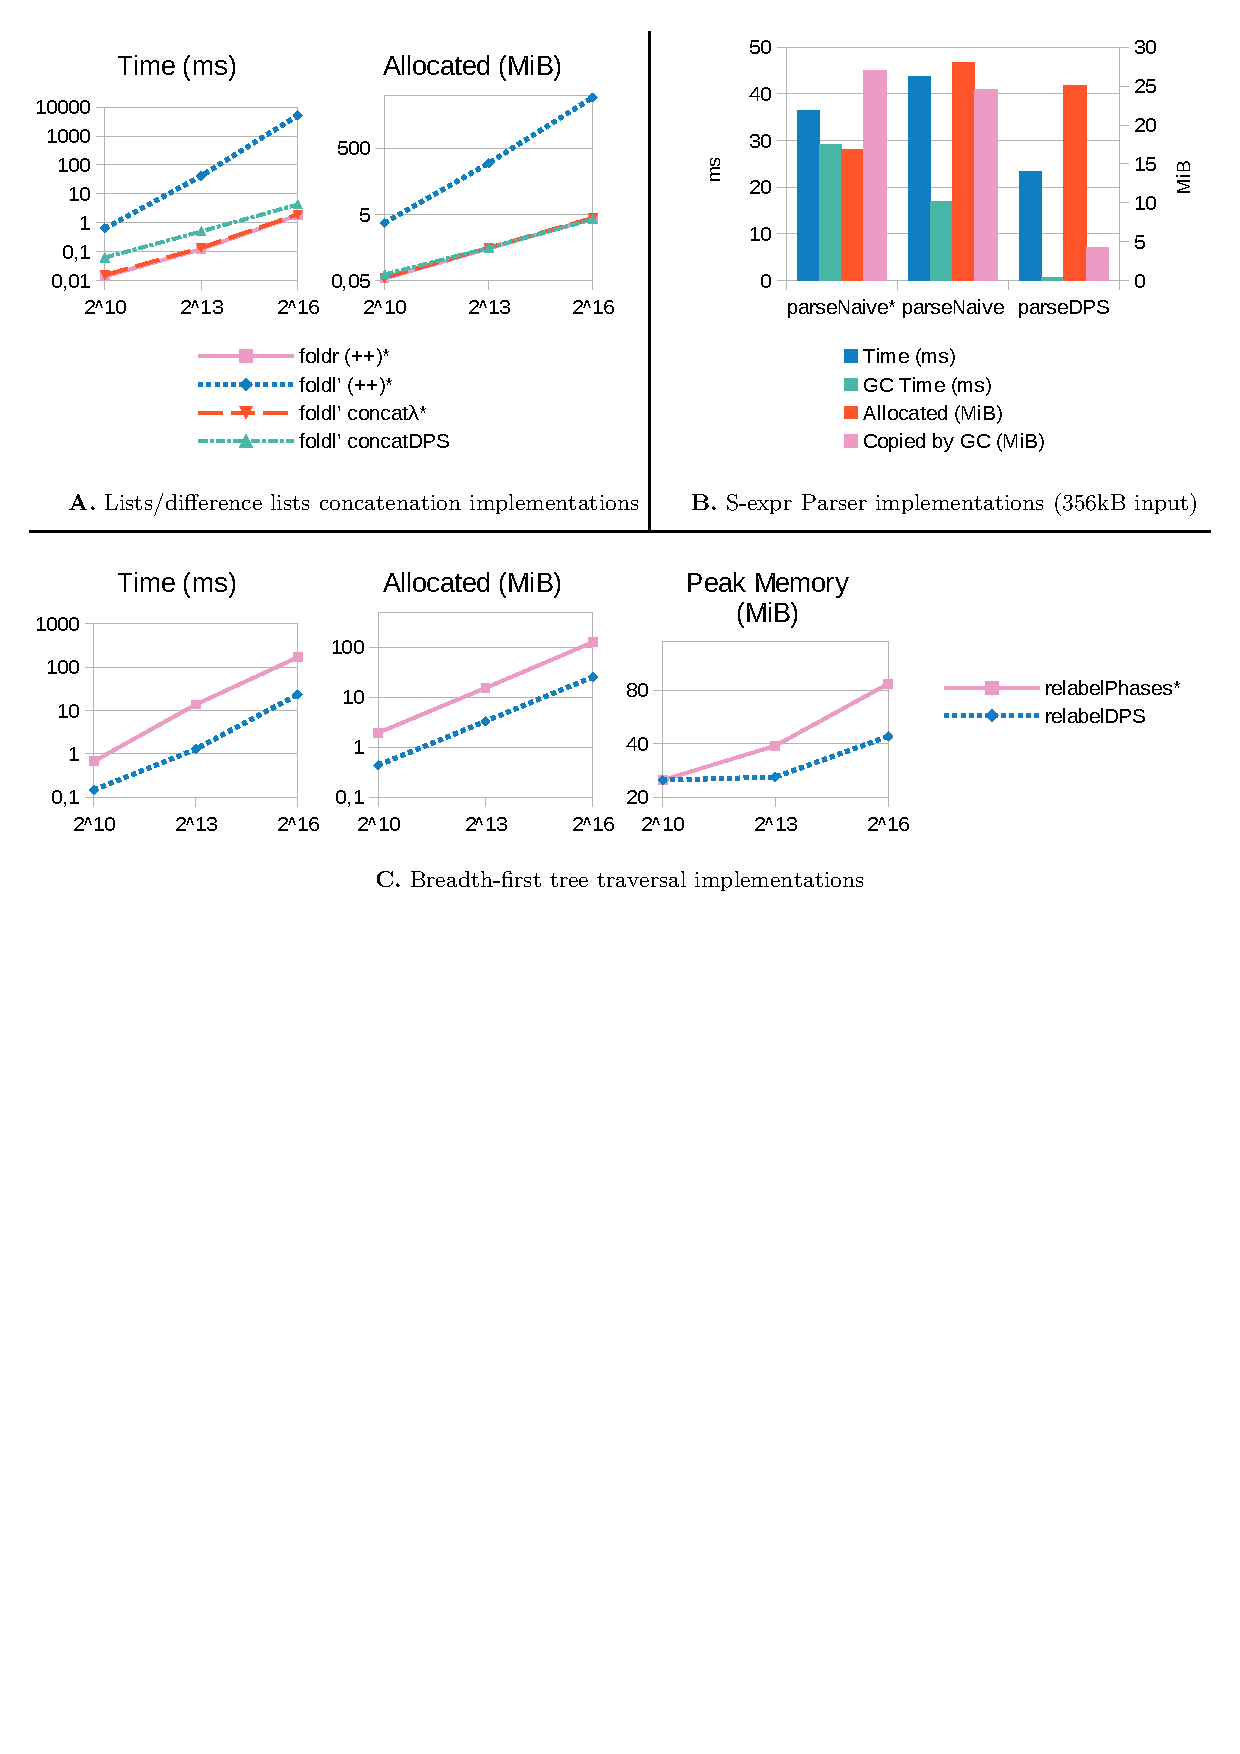
\includegraphics[width=14cm]{bench-charts.pdf}
  \caption{Benchmarks ran on AMD EPYC 7401P @ 2.0 GHz (single core, \texttt{-N1 -O2})}
  \label{fig:bench-charts}
\end{figure}

\subsection{Concatenating lists and difference lists}\label{ssec:benchmark-dlist}

We compared four implementations:
\begin{itemize}
\item \mintinline{haskell}`foldr (++)` where calls to \mintinline{haskell}`(++)` are nested to the right, giving the most optimal context for list concatenation (it should run in $\mathcal{O}(n)$ time)
\item \mintinline{haskell}`foldl' (++)` which is the worst case for list concatenation, expected to run in $\mathcal{O}(n^2)$ time.
\item \mintinline[escapeinside=°°]{haskell}`foldl' concat°$\lambda$°` which uses function-backed difference lists, and \mintinline{haskell}`foldl' concatDPS` which uses destination-backed difference lists. Both are expected to run in linear time even if the concat calls are nested to the left.
\end{itemize}

We see in part 1 of figure~\ref{fig:bench-charts} that the destination-backed difference lists have a comparable memory use as the two other linear implementations, and a very slight edge for large data sets (5-10\% fewer allocations), in exchange for being quite slower (2-4$\times$ time).


\subsection{Relabeling a tree in a breadth-first fashion}\label{ssec:benchmark-bf-tree-traversal}

We see in part 2 of figure~\ref{fig:bench-charts} that the destination-based tree traversal is almost one order of magnitude more efficient, both time-wise and memory-wise, compared to the implementation based on \emph{Phases} applicatives presented in~\cite{gibbons_phases_2023}.

\subsection{Parsing S-expressions}\label{ssec:benchmark-parser}

In part 3 of figure~\ref{fig:bench-charts}, we compared the ``naive'' implementation of the S-expression parser (presented in table~\ref{table:impl-sexpr-parser-without-dest}) and the DPS one (presented in table~\ref{table:impl-sexpr-parser-with-dest}) ran against a 15,000-lines-long Lisp file.

It is interesting to see that the DPS version makes about 50\% more allocations than the starred naive version, but uses 10\% less memory at its peak (not shown in the figure), and more importantly, spends 38$\times$ less time in garbage collection (with 6$\times$ less bytes copied by the GC). As a result, the DPS version only takes 0.55-0.65$\times$ the time spent by the naive version, mostly thanks to garbage collection savings. This also indicates that most of the data allocated in the garbage-collected heap by the DPS version just lasts one generation and thus can be discarded very early by the GC, without needing to be copied into the next generation, unlike most nodes allocated by the naive version.

We can also observe in part 3 of figure~\ref{fig:bench-charts} that copying the result of the naive version in a compact region (which can be desirable for future GC savings, as detailed in subsection~\ref{ssec:parser-sexpr}) makes it even longer, and results in even more total allocations than DPS version.

This benchmark is probably the most significant of the paper: it proves that DPS is a viable technique for some real-world use cases, bringing gains that cannot be obtained easily with other approaches in pure functional programming languages.

\subsection{Mapping a function over a list}\label{ssec:benchmark-map}

It seemed important to also measure the performance of a \mintinline{haskell}`map` function implementation using destinations. In a strict functional language such as OCaml, the choice of implementation for \mintinline{haskell}`map` is crucial as the naive one makes the stack grow linearly with the size of the processed list. A strict tail-recursive version (\mintinline{haskell}`mapTR'`) takes $\mathcal{O}(1)$ space, but it requires an extra $\mathcal{O}(n)$ operation at the end of the processing (reversing the accumulator). 

With destinations, \mintinline{haskell}`map` can be implemented in a tail-recursive fashion without the need for the reverse operation (as the list is built in a top-down approach). It can also be implemented as a fold:
{\small
\begin{minted}[linenos]{haskell}
append :: Dest [a] ⊸ a → Dest [a]
append d x = let !(dh, dt) = fill @'(:) d in fillLeaf x dh ;; dt

mapDPS' _ [] d = fill @'[] d
mapDPS' f (x : xs) d = let !r = f x ; !d' = append d r in mapDPS' f xs d'

mapDPSFold' f l dl = fill @'[] (foldl' (\d x → let !r = f x in append d r) d l)
\end{minted}
}

We see in part 4 of figure~\ref{fig:bench-charts} that the destination-based implementations takes 1.5-4$\times$ more time than \mintinline{haskell}`map` and \mintinline{haskell}`mapTR'` (depending on the dataset size), but memory-wise both \mintinline{haskell}`mapDPS'` and \mintinline{haskell}`mapDPSFold'` are more efficient than \mintinline{haskell}`map`; and \mintinline{haskell}`mapDPS'` even manage to make 13\% fewer allocs than \mintinline{haskell}`mapTR'` on the largest dataset.

In OCaml, it is important to note that \mintinline{haskell}`mapDPS'` is actually more performant time-wise than \mintinline{haskell}`mapTR'` ($0.5-0.85\times$) even for small lists, as detailed in~\cite{bour_tmc_2021}.

\section{Related work and future developments}

The idea of functional data structures with write-once holes is not new. Minamide already proposed in~\cite{minamide_functional_1998} a variant of $\lambda$-calculus with support for \emph{hole abstractions}, which can be represented in memory by an incomplete structure with one hole and can be composed efficiently with each other (as with \mintinline{haskell}`fillComp` in figure~\ref{fig:schema-dlist-concat}). With such framework, it is fully possible to implement destination-backed difference lists for example, as we developed in subsection~\ref{ssec:dlist}.

However, in Minamide's work, there is no concept of destination: the hole in a structure can only be filled if one has the structure itself at hand. On the other hand, our paper introduces destinations, which are a way to interact with a hole remotely, even when one doesn't have a handle to the associated data structure. Because destination are treated as first-class objects, they can be passed around or stored in collections or other structure. Being able not only to represent data structures with holes, but also manipulate references to these holes as first-class objects and storing them in arbitrary containers (as in subsection~\ref{ssec:bf-tree-traversal}) while preserving memory safety, is the major step forward that this paper presents.

More recently, \cite{protzenko_mezzo_2013} introduced the Mezzo programming language, in which mutable data structures can be freezed into immutable ones after having been completed. This principle is used to some extend in their list standard library module, to mimic a form of DPS programming, albeit it cannot easily express one-pass breadth first traversal or one-pass tail-recursive map as in subsections~\ref{ssec:bf-tree-traversal} and~\ref{ssec:benchmark-map}. An earlier appearance of DPS programming as a mean to achieve better performance in a mutable language can also be seen in~\cite{larus_restructuring_1989}.

Finally, both \cite{shaikhha_destination-passing_2017} and \cite{bour_tmc_2021} use DPS programming to make list or array processing algorithms more efficient in a functional, immutable context, by turning non tail-recursive functions into tail-recursive destination-based ones, as we did in~\ref{ssec:benchmark-map}. More importantly, they present an automatized way to go from a naive program to its tail-recursive version. However, holes/destinations are only supported at an intermediary language level in those papers, whereas both~\cite{minamide_functional_1998} and our current work support safe DPS programming in user-land.

\section{Conclusion and future work}

Programming with destinations definitely has a place in the realm of functional programming, as the recent adoption of \emph{Tail Modulo Cons}~\cite{bour_tmc_2021} in OCaml compiler shows. In this paper, we have shown how destination-passing style programming can be used in user-land in Haskell safely, thanks to a linear type discipline. The associated implementation relies only on a few alterations to the compiler, thanks to \emph{compact regions} that are already available as part of GHC. Adopting DPS programming opens the way for more natural and performant programs in a variety of contexts, where the major points are being able to build structures in a top-down fashion, manipulating and composing incomplete structures, and managing holes in these structures as first-class (destinations). Simultaneously, our implementation allows to efficiently build structures in \emph{compact regions}, which wasn't possible before.

There are two main limitations that we would like to lift in the future. Firstly, DPS programming could be useful outside of compact regions: destinations could probably be used to manipulate the garbage-collected heap (with proper read barriers in place), or other forms of secluded memory areas that aren't traveled by the GC (RDMA, network serialized buffers, etc.). Secondly, we would like to store linear data through destinations: in the breadth-first tree traversal, we then would be able to store destinations (which are linear resources) inside a destination-backed queue for extra efficiency. At the moment the signature of \mintinline{haskell}`fillLeaf` restricts this usage. The deeper reason is that with destination-backed containers (unlike constructor-backed ones), one can make an object escape from the current scope into the parent one, while marking it has having been consumed. This isn't a problem for non-linear objects, but it is for destinations (viewed as linear objects): their consumption must always be linked with a hole being filled, but this is not what directly happens if a destination is stored away in the parent scope. We probably need a more refined API and/or type system to allow that without breaking memory safety.

\printbibliography

\end{document}
